\section{MediaScope}
\label{sec-3}

\begin{figure*}[t]
  \begin{minipage}{0.32\linewidth}
    \centering \epsfig{file=pics/cdf.eps, width=0.96\linewidth}
    % \vspace{-1mm}
    \caption{CDF of Flickr Photo Availablility Gap}
    %\vspace{-6mm}
    \label{fig:cdf}
  \end{minipage}
  \begin{minipage}{0.32\linewidth}
    \begin{center}
      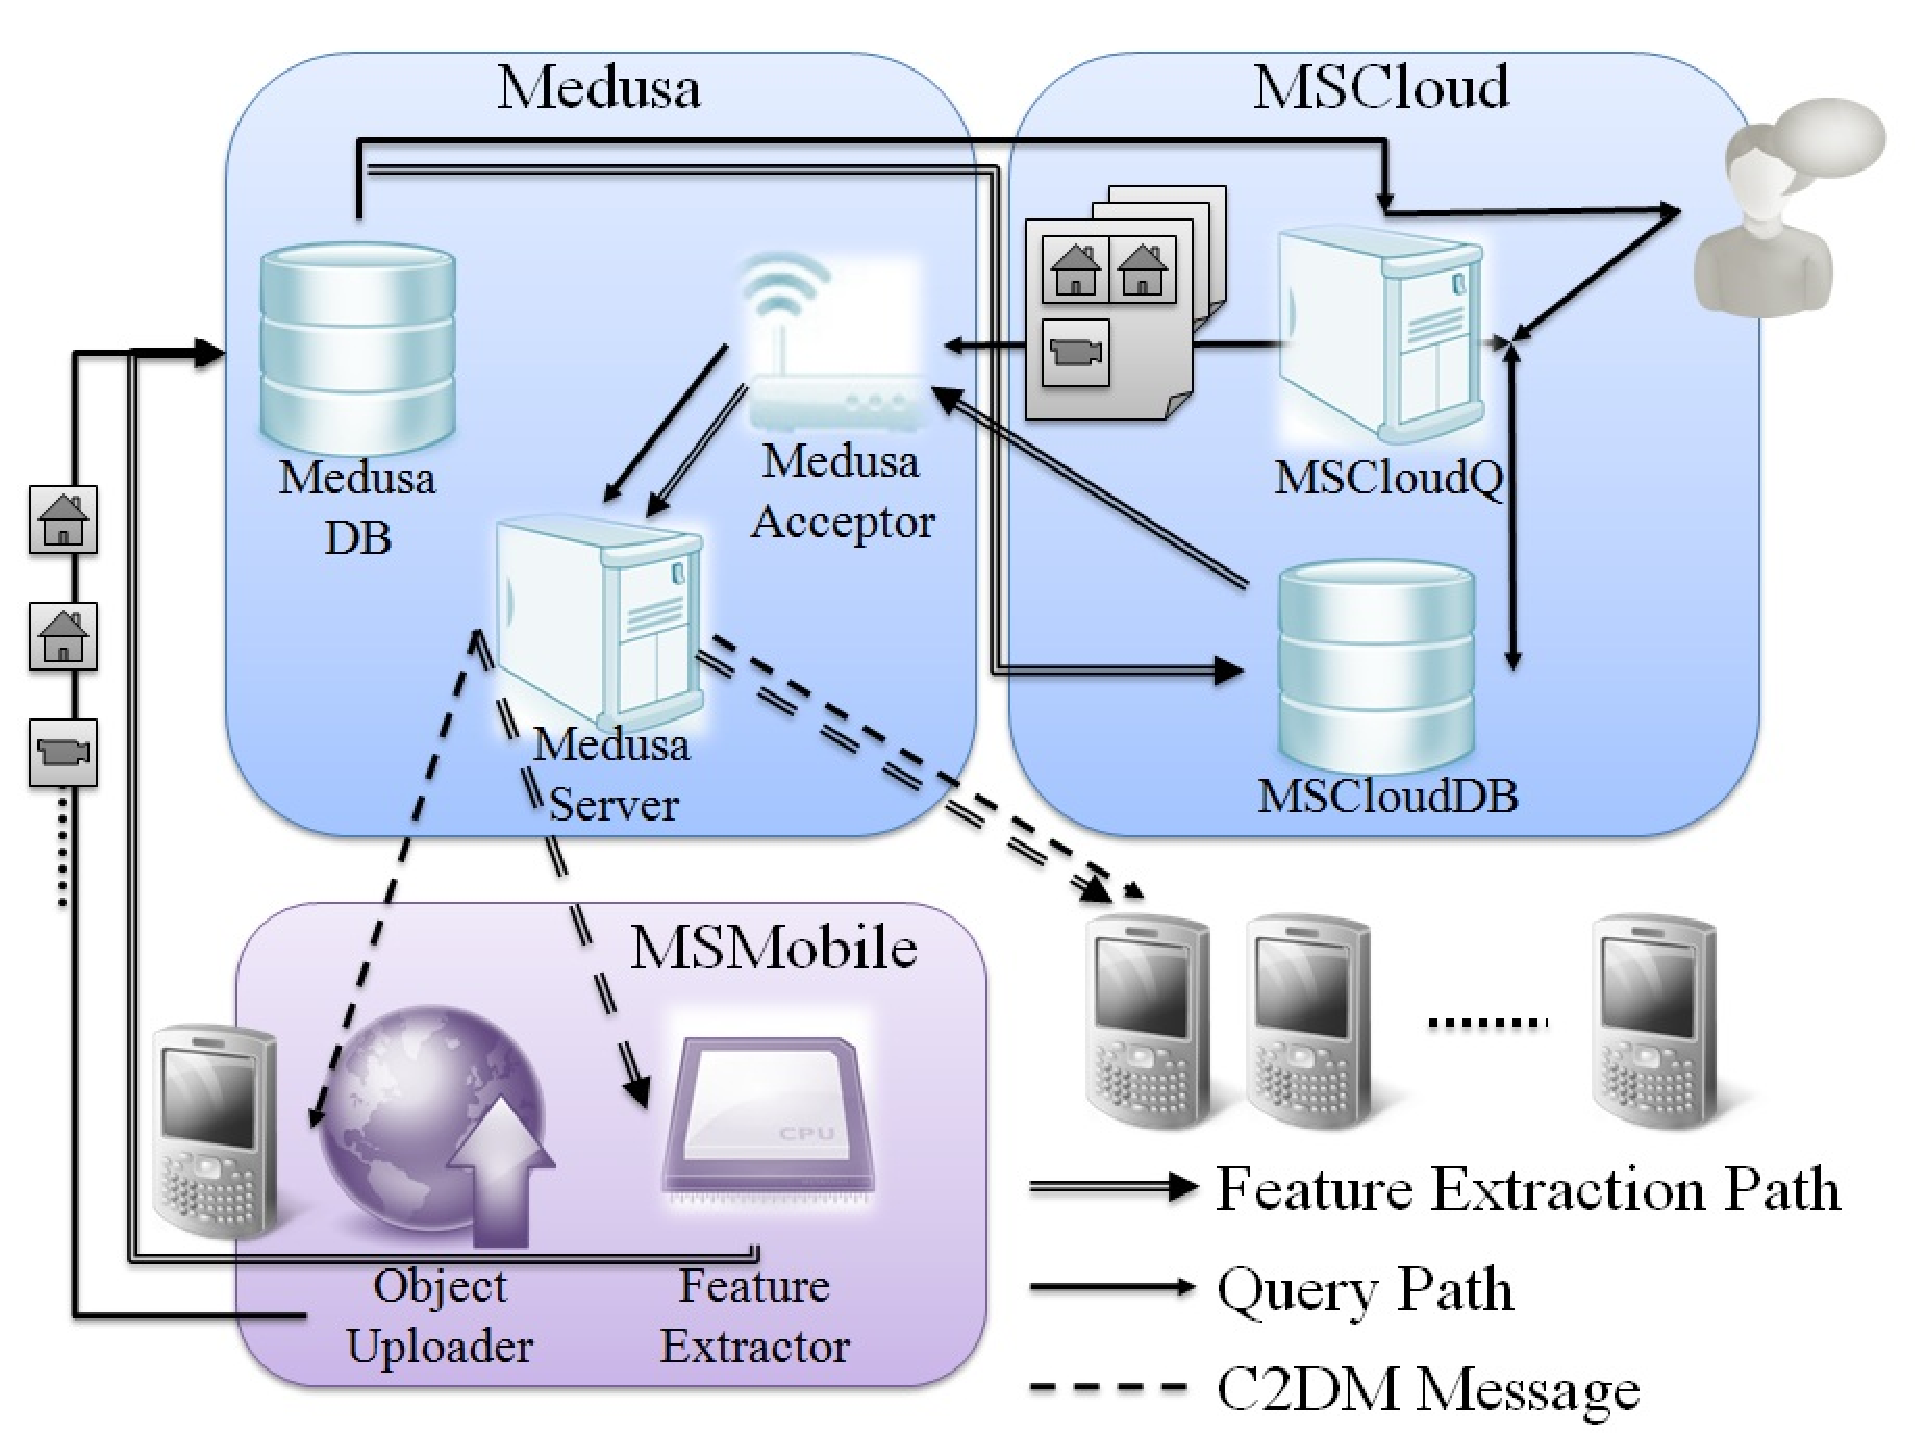
\epsfig{file=pics/architecture.eps,width=0.96\linewidth}
    \end{center}
%    \vspace{-6mm}
    \caption{System Architecture Work Flow}
%    \vspace{-6mm}
    \label{fig:architecture}
  \end{minipage}
  \begin{minipage}{0.32\linewidth}
      \begin{center}
        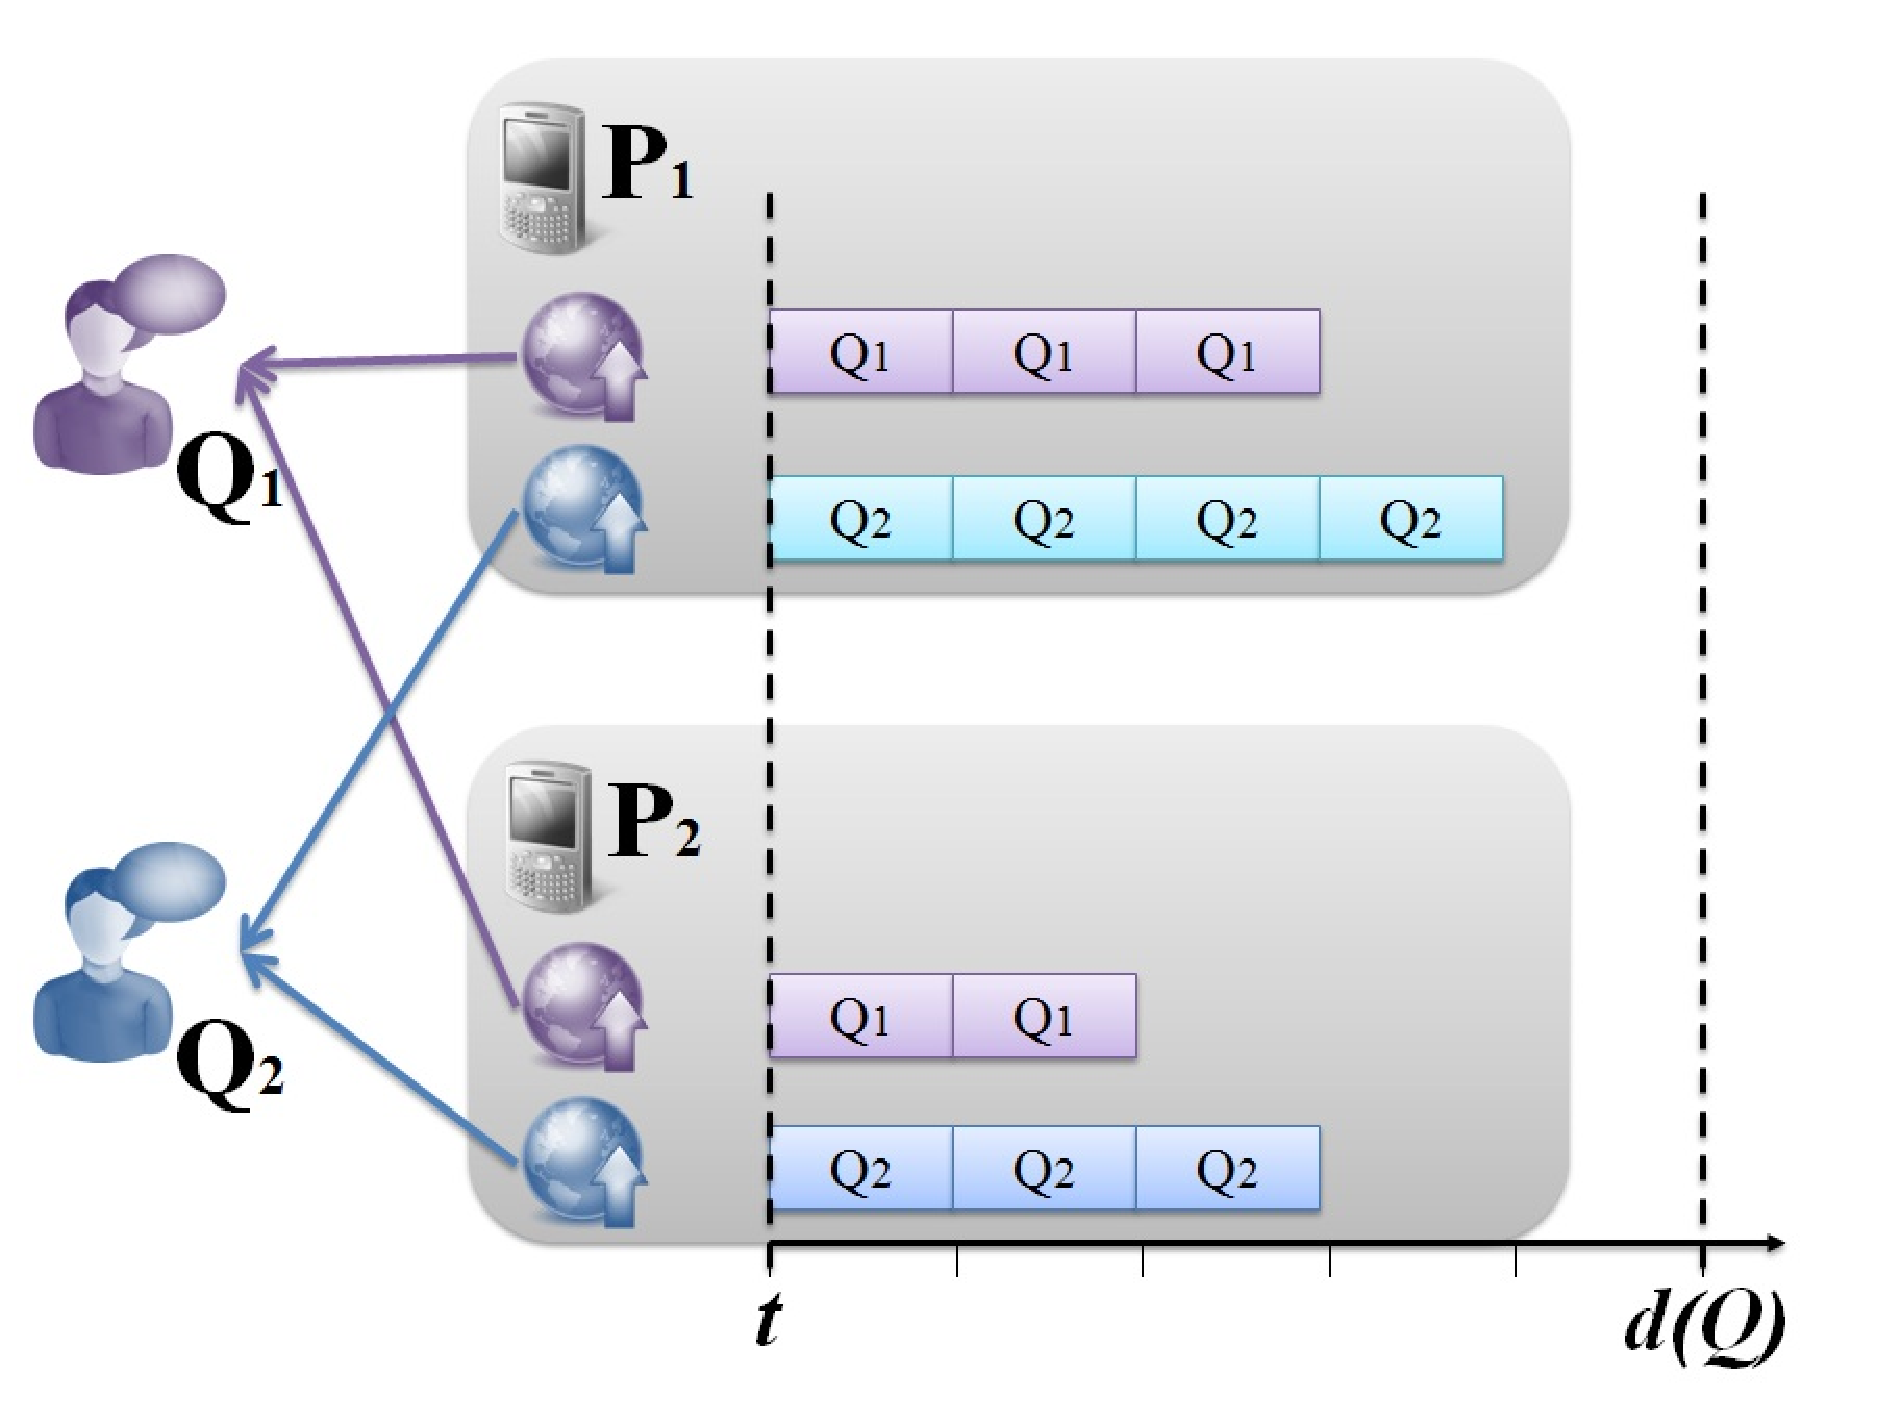
\epsfig{file=pics/example.eps,width=0.96\linewidth}
      \end{center}
%      \vspace{-6mm}
      \caption{Illustration of Concurrent Queries}
%      \vspace{-6mm}
      \label{fig:example}
    \end{minipage}
\end{figure*}

MediaScope is a system that supports timely similarity-based queries
on media objects stored on mobile devices.
%
We begin by describing the MediaScope architecture and then discuss
the design and implementation of each component.

%\vspace*{-0.75ex}
\subsection{Architecture and Overview}
\label{sec-3-1}

Mediascope is conceptually partitioned across a cloud component called
MSCloud, and another component called MSMobile that runs on mobile devices.
%
This partitioned design leverages the computation and storage in
clouds to support geometric queries on the feature space; mobile
devices provide sensing and storage for media objects.

These components interact as follows (Figure~\ref{fig:architecture}).
%
Whenever participants take photos or videos, the \emph{Feature
  Extractor} component of MSMobile continuously extracts, in the
background, image and video features and uploads them to the
\emph{MSCloudDB}.
%
Users (e.g., a security officer or a sportswriter) pose queries to MSCloud
using a standard web interface, possibly on a mobile device.
%
These queries are processed by the \emph{MSCloudQ} query processing
engine, which uses the features stored in the MSCloudDB to compute the
query results.
%
The results of the queries identify the media objects that need to be
retrieved from individual mobile devices.
%
In some cases, a media object may already have been retrieved as a
result of an earlier query; query results are also \emph{cached} in
MSCloudDB in order to optimize retrieval.
%
MSCloudQ coordinates with an \emph{Object Uploader} component on
MSMobile in order to retrieve query results.
%
\camera{Once a query's timeliness bound expires, MSCloudQ terminates
  the corresponding Object Uploader and returns retrieved results.}

MediaScope uses a publicly available crowd sensing platform called
Medusa~\cite{Medusa}.
%
Medusa was originally designed to permit human users to pose
crowd-sensing tasks.
%
MediaScope's retrieval of features and media objects from mobile
devices leverages Medusa's support for ``sensing'' stored information
on these devices.
%
To enable programmed interaction between MSCloud and Medusa, and to
support MediaScope's timeliness requirements, we made several
modifications to the Medusa platform (discussed later).

MediaScope thus provides a high-level abstraction (queries on media
objects) that hides many of the details of object retrieval from
users.
%
In the following subsections, we describe the two most challenging
aspects of MediaScope design: \emph{support for concurrent queries},
a functionality distributed between the MSCloudQ and the Object
Uploader; and \emph{feature extraction}.
%
We conclude with a brief description of other design and
implementation issues.

% First, on MSMobile, there is media file observer which stores all existing media objects (photos and videos)'s general metadata, periodically, MSMobile will execute a media object feature generation task, which compute the feature vectors for each media object, and uploads them to MSCloud. One advantage is that through this way, we avoid the uploading of original media files, which will significantly save the users' bandwidth, e.g. in our implementation, generally one image's original size is about 1.5MB, but the feature data we need to upload is only 54B, for a high definition 30s video taken by Galaxy SIII is about 63M, we only need to upload less than 10 features of the video which is only 540B. Second advantage is that, with a same feature extraction algrithm on the phone as on the cloud, we won't loss any accuracy of these feature metadata.

% Second, interface to commander is clean and concise. Commanders pose search queries of their interest, through the interface to interact with MSCloud. The rest of all the work is left to MSCloud, which will complete all necessarily processing and tasks in the background. MSCloud has two components.
% \begin{itemize}
% \item \textbf{MSCloudDB}: First, Media objects' features uploaded from phones are stored here. It is able to support multiple phones concurrent uploading features at same time, as well as multiple queries concurrent data retrieval. Second, queries' results (original media files) uploaded from phones are also stored here. Since we want to reuse already uploaded media files, MSCloudDB also support media feature data realtime update.
% \item \textbf{MSCloudQ}: MSCloudQ is the query processing engine on the cloud, which includes:
% \begin{itemize}
% \item Interface to Commander. Commander is not necessary to understand the background mechanisms, we provide a detailed query type explaination and straghtforward parameter options for commander. Once the deadline hits or resources are ready, it will pick up the corresponding media files from MSCloudDB, and respond to commander.
% \item Query resolver, and query algorithm execution. Its job is to understand the query objective and parameters, retrieve the data from MSCloudDB, pass them to query optimizer, which will consider all the reality situation and available resources, output the need-to-upload list for each involved users.
% \item Interaction with Phones. After receiving the upload list from query optimizer, MSCloudQ will write task script for each phone, including the uploading scheme parameters, and wait the task execution results from the phone. This part is aware of the deadline of the query, so it will automatically notify the front end interface the file locations, as well as the task termination on the phone.
% \end{itemize}
% \end{itemize}

% Third, MSMobile will accept task notifications from MSCloudQ with task desciption, which are all quite lightweight, usually less than 1Kbytes. MSMobile has its own file uploading scheme, called \emph{maximum credit scheme}, we will discuss it in detail in following.



% In summary, our system work flow is shown in Figure~\ref{fig:architecture} (will be modified to new architecture image).
%%

%\vspace*{-0.75ex}
\subsection{Design: Concurrent Queries}
\label{sec-3-2}

The most challenging component of MediaScope is support for concurrent
queries~---~\camera{MSCloudQ may receive one or more queries while
  other queries are being processed.}
%
In MediaScope, the result of a query is a list of media objects to be
retrieved from a subset of the participating phones.
%
Recall that each query has a timeliness constraint.
%
In the presence of concurrent queries, MediaScope may need to upload
all media objects before their timeliness bound expires.
%
In general, this may be difficult to achieve because \camera{wireless
bandwidth can vary significantly over time, resulting in variable
upload times for images.}

To illustrate this, consider the example of two concurrent queries
$Q_1$ and $Q_2$ that arrive at the same time for media objects
distributed across two phones $P_1$ and $P_2$ in Figure~\ref{fig:example}.
%
Also, assume that both queries have a timeliness bound of 5 seconds,
each object can upload 1 object per second, and all objects are of the
same size.
%
If $Q_1$ needs to retrieve 3 objects from $P_1$ and 2 objects from
$P_2$, while $Q_2$ needs to retrieve 4 objects from $P_1$ and 3 from
$P_2$.
%
Under these circumstances, it is not possible to satisfy the
timeliness requirements of
%\xing{both?} No, there exists a schedule by which either q1 or q2 can
%be satisfied, but not both
one of the two queries.
%
In practice, the problem is much harder because there may be more than
two concurrent queries, many more participating devices, queries can
arrive at different times, media objects may have different sizes, and
wireless available bandwidth can vary dynamically.
%
Especially because of the last reason, \camera{admission control
  cannot guarantee that all timeliness constraints are met, or may
  severely underutilize the available bandwidth}.

MediaScope uses a different approach, \emph{trading off query
  completeness for timeliness}.
%
In MediaScope, not all query results may be uploaded within the
timeliness bound, but the challenge is to upload the most relevant
queries so as to maximize the amount of \emph{information} retrieved.
%
In doing this, there are two challenges: how to differentiate between
queries, and how to prioritize media items for the retrieval in order
to maximize the information retrieved.

% In this case, our goal is to attempt to maximize the amount of
% information delivered across all queries. In particular, this means
% that it would be preferable to obtain as much of the ``high order bits''
% of the query result for each query, than to obtain all of the results
% for one query.

MediaScope addresses these two challenges using a \emph{credit
  assignment} mechanism.
%
Each query is assigned, by MediaScope, a number of credits.
%
The credits assigned to a query reflect the importance of that query
and result in proportionally more information being uploaded for that
query (and therefore the proportional completeness of the query result).
%
The specific credit assignment mechanism for queries is beyond the
scope of this paper, but MediaScope may use monetary incentives (e.g.,
users who pay more get more credits \camera{for their queries}) or other
approaches in order to assign credits to queries.

If a query is assigned $n$ credits, it divides up these credits among
its results (media objects) in a way that reflects the importance of
each object to the query.
%
The key intuition here is that, for a given query, \camera{\emph{the
  importance of a result object to the query can be determined by the
  feature space geometry}}.
%
For example, consider a query $Q$ which attempts to retrieve the two
nearest photos in feature space to a given photo $c$.
%
If the resulting photos $a$ and $b$ are each 20 units and 80 units
distant from $c$ in feature space, and $Q$ has been assigned 100
credits, $a$ and $b$ each receive 80 and 20 credits respectively (in
inverse proportion to their distances to $c$).
%

MediaScope uses this intuition to define credit assignment to result
objects.
%
Once objects have been assigned credits, object uploading is
prioritized by credit in order to maximize the total credit retrieved
across all concurrent queries.
%
In what follows, we first describe the queries that MediaScope
supports and how credits are assigned for each query.
%
We then describe MediaScope's credit-based object scheduling technique
and discuss its optimality.

% Our approach uses two mechanisms to address this challenge:
% \begin{itemize}
% \item a system defined assignment of ``credits'' to individual queries: this
%   assignment roughly determines the relative proportion of resources
%   that this query can use, that is, any query $Q_i$ has been assigned the credits $c(Q_i)$.
% \item for each query, we also define a method by which credits can be
%   allocated to query results and design a scheduling algorithm that
%   attempts to maximize the total number of credits retrieved. For example, $n$ objects best answers query $Q_i$, namely $Q_i=\{o_i^1, o_i^2, \cdots, o_i^n\}$, we assign $n$ objects with credits $c(o_i^1), c(o_i^2), \cdots, c(o_i^n)$ and satisfy $c(Q_i)=\sum_{o\in Q_i} c(o)$
% \end{itemize}

% Thus, query semantics are ``approximate'' necessarily because of
% timeliness constraints one may not get complete queries; level of
% completeness can be varied by adjusting the credits assigned to each query.

%\vspace*{-0.75ex}
\subsubsection{Queries and Credit Assignment}
\label{sec-3-2-1}

Our current instantiation of MediaScope supports three qualitatively
different queries: nearest neighbor, clusters, and spanners.
%
Below, we discuss the design of the query engine MSCloudQ and how
credits are assigned to query results.
%
Recall that for each query, users can specify time, location and
freshness attributes: before performing each of the queries described
below, MSCloudQ filters all the feature vectors stored in MSCloudDB to
select feature vectors that match these attributes.
%
In our description of the queries below, we assume that this filtering
step has been applied.

% We are supporting four queries from the discussion of \ref{sec-2-2}.
% %
% In order to fullfill different query requirement, we design specified
% algorithms for each query that best coordinate the idea of the query.
% %
% Algorithm for each different query not only generates a list of media
% objects to upload, but each media object is associated with a credit,
% indicating the “importance” of such object.
% %

% We introduces the design for different queries, each query is associated with two steps: first, query optimization(algorithm execution), second, credit assignment.

\mypar{k-Nearest Neighbors.}
%
For this query, the user supplies a \emph{target} image and the server
attempts to return the $k$ nearest images (from photos or videos) in
feature space to the target.
%
The implementation of this query is straightforward: it is possible to
build indexes to optimize the search for the $K$ nearest neighbors,
but our current implementation uses a brute force approach.

% \textbf{Step 1}: The algorithm for this query is quite straghtforward, MSCloudQ first filters out those not qualified metadata from MSCloudDB, and returns qualified media metadata, \emph{Top K algorithm} iterates over all qualified feature data, calculate the given image's feature similarity to those from MSCloudDB, and returns Top K similar objects' IDs to MSCloudQ.

Credit assignment for this query attempts to capture the relative
importance of the query results.
%
Thus, the assignment of credits to each result is proportional to its
similarity to the target image.
%
For the $i$-th result, let $s_i$ be the similarity measure to the
target; we then assign credits to the $i$-th result proportional to
$p_i = (1 - \frac{s_i}{\sum{s_i}})$.

%
% So our assigning scheme is to assign credit proportional to the
% similarity to the original given image.
% %
% Specifically, take similarity value for each object from the intended
% object, denote as $s_{i}$, the smaller $s_i$, the more similar, so the
% portion is
%

\mypar{$K$ Clustering.}
%
The second class of queries supported by MSCloudQ is based on
clustering in feature space.
%
This query takes as input the number $k$ as well as well as a
\emph{type} parameter which describes the expected result and can have
one of two values:
\begin{description}
\item[Cluster Representative] With this parameter, the result contains
  $k$ images, one from each cluster. For each cluster, our algorithm
  selects that image as the representative whose distance is least to
  the centroid of the cluster. Intuitively, this query type identifies
  different ``topics'' among images taken by participating users.
\item[Common Interest] With this parameter, the result includes images
  from that cluster which contains objects belonging to the most
  number of users. Thus, if the $i$-th cluster contains images from
  $u_i$ users, the query returns images from that cluster for which
  $u_i$ is the largest. Intuitively, this query identifies the cluster
  that represents the maximal common interest between participating
  users. Within the selected cluster, the query returns one image for
  each participating user, selecting that image of the user that is
  closest to the centroid of the cluster.
\end{description}
%
These queries can be implemented by any standard algorithm for
$k$-means clustering.

For the \emph{cluster representative} type of query, we assign credits
proportional to the size of the cluster.
%
Thus, if the $j$-th cluster's size is $c_j$, the credit assigned to
the image selected from cluster $j$ is proportional to $\frac{c_j}{\sum{c_j}}$.

For the \emph{common interest} type of query, we assign a credit to
each selected image that is inversely proportional to the image's
distance from the centroid of the cluster.
%
The credit assignment is similar to $k$ nearest neighbors above.

% Second query we proposed is \emph{K Representative Objects} , with which, people can find out K most representative objects over the whole database.

% \textbf{Step 1}: We tried few algorithms for  \emph{K Representative Objects} Query. The way we evaluation the algorithm performance is that we manually took around 200 photos in 5 different scenes of 5 different locations with Galaxy SIII, manually marked those 200 photos into 5 clusters. Then we apply different clustering algorithm on the dataset, and compare the results with manually marked clusters. We found that \emph{KMeans} clustering performs best with an average less than 2 error photo classification  per cluster. So the final algorithm we adopted for this query is  K-Means algorithm. After retrieving related feature data from MSCloudDB, we use Kmeans to classify the all qualified objects to $K$ clusters, and select one object from each cluster under the condition that the object is most close(similar) to its cluster center.

% \textbf{Step 2}: The concept of credit assigment here is a little different from previous query, similarity here is not a good metric anymore, since only one object is selected in each cluster. We proposed the cluster size metric which indicates that the larger a cluster, the more credit the representative object should get.  So consider cluster $i$'s size $cs_i$, the credit portion for cluster $i$ is $\frac{cs_i}{\sum{cs_i}}$ and assign credit according to the proportion.

% Third query we proposed is \emph{Common Interest Objects}: people might want know others' common interest, e.g. most people tend to  take photos or videos of some sightseeing, like beach, ocean, if most people has such interest, we can point it out and show these photos or videos to commander.

% \textbf{Step 1}: The algorithm here is same as \emph{K representative objective} query, we use KMeans to clusters qualified features to $K$ clusters(we predefined the parameter $K= 6$ in the algrithm, commander is free to assign or not ). The difference compared to previous query is that we will select the cluster with most different users, if multiple clusters have same number of users involved, we use number of objects as another criteria. We will return the objects in selected cluster.

% \textbf{Step 2}: Here, our idea for credit assigment is that more close to cluster center, more credit it should get, we assign like this is because those close to center objects contains more information compared to those who are far from center. The rest is identical to the algorithm in \emph{Top K Objects} Query.

\ifdefined\notdef
\mypar{Spanner.}
%
The third query that MediaScope supports is based on spanning the
feature space.
%
The intuition behind the query is to return a collections of images
which \emph{span} the feature space.

% Forth query in our system is \emph{Spanner: Most distinct object Set}, the intuition behind this query is that commander may be interested in the total information contained by the available data. To select a set of media objects that contains most information requires those objects to be quite distinct to each other. So for this query, we first defined in a rigorous mathematical way, and give a suboptimal algorithm to the problem.

MSCloudQ uses a maximum weighted spanning tree algorithm in order to
select results for this query; it attempts to find the most dissimilar
pairs of objects from each participating user, while constraining the
number of images selected from each user to a nominal ``budget''.
%
Assume that $K_n$, the complete graph on $n$ vertices (vertices
represent objects), has a vertex set $V$ which is partitioned into $C$
classes $V_{1},\ldots,V_{C}$ (classes represent users).
%
Let $v_{i_t}$ denote vertex $i$ in class $V_t$.
%
Let $e_{i_t j_k}$ represent the edge connecting $v_{i_t}$ with
$v_{j_k}$.
%
Assume edge $e_{i_tj_k}$ has weight $w_{i_tj_k}$ (where the weight
represents the dissimilarity between objects $i_t$ and $j_k$).
%
Furthermore, assume vertex $i_t$ has size $s_{i_t}$ (size of object
$i_t$), and class $j$ has capacity $b_j$ (total size that can be
uploaded from user $j$).
%

The objective is to find a spanning tree of maximum weight on a vertex
subset which respects the class size constraints.
%In this case, we can easily prove that the added edge value decreases with adding order.
%The physical meaning behind this objective is that the
%selected points are as distinct to each other as possible.
This objective selects objects which are dissimilar from one
another.
%
Here is the integer program for this problem:

{\footnotesize
\begin{align}
\max        & \notag
              \sum_{i_t< j_k} w_{i_tj_k} y_{i_tj_k} \\
\text{s.t.     } & \label{con:ineq1}
              y_{i_tj_k} \leq x_{i_t}             & \forall i_t\neq j_k \\
            & \label{con:ineq2}
              y_{i_tj_k} \leq x_{j_k}             & \forall i_t\neq j_k\\
            & \label{con:ineq4}
            \sum_{i_t\in V_t} s_{i_t}x_{i_t}\le b_t        & \forall t=1,\ldots , C \\
            & \label{con:ineq5}
            \sum_{i_t<j_k} y_{i_tj_k}=\sum x_{i_t}-1      &    \\
             & \label{con:ineq6}
            \sum_{i_t<j_k} y_{i_tj_k}\le |S|-1           & \forall S\subset V, S\neq \emptyset\\
            & \notag
            x_{i_t} \in\{0,1\}        & \forall i_t\\
            & \notag
            y_{i_tj_k} \in\{0,1\}                 & \forall i_t\neq j_k
\end{align}
}

In this integer program, variable $x_{i_t}$ is used as the indicator
variable for selecting vertex $v_{i_t}$.
%
Similarly, variable $y_{i_tj_k}$ is used as the indicator variable for
selecting edge $e_{i_tj_k}$.
%
Inequality \ref{con:ineq1} and \ref{con:ineq2} ensure that edge
$e_{i_tj_k}$ is not selected if either vertex $i_t$ or $j_k$ is not
selected.
%
Inequality \ref{con:ineq4} ensures that the total size of vertices
chosen from class $V_i$ does not exceed $b_i$.
%
Denotation \ref{con:ineq5} and \ref{con:ineq6} ensures that a maximum
spanning tree is selected.
%
Since the above problem is NP-hard, we use a $O(N^2log(N)^2)$
heuristic (Algorithm~\ref{alg:mst}).
%

For this query, intuitively, credit assignment should give more
importance to dissimilar images.
%
For the $i$ query result, we compute $d_i$, the average distance from
the $i$-th image to all other images.
%
The credit assigned to this image is proportional to
$\frac{d_i}{\sum{d_i}}$. %\ramesh{Please check.}\jyr{I didn't find problem here}

% \textbf{Step 2}: From the above algorithm we get a set of media objects that most dissimilar to each other. Our design for the credit assignment is that take average similarity to all other selected objects as the metric for each objects, say for object $i$ that average similarity to other objects is $avgsim_i$, and its credit portion is $\frac{avgsim_i}{\sum{avgsim_i}}$ the credit assignment is according to the portion. The meaning for this assigment is that those who are farest from others need more credit because it contains the information that might quite independent to others.

% Algorithm for each different query not only generates a list of
% media objects to upload, but each media object is associated with a
% credit, indicating the ``importance'' of such object. We can
% evaluate each query's result as the total credits of uploaded media
% objects.

\fi

\mypar{Spanner.}
%
The third, and qualitatively different query that MediaScope supports
is based on spanning the feature space.
%
The intuition behind the query is to return a collection of images
which \emph{span} the feature space.
%
In computing the spanner, we assume that each user $t$ contributes
exactly $s_t$ images, where $s_t$ is derived from the query's
timeliness bound and a nominal estimate of the average upload rate
from the corresponding mobile device\footnote{ \camera{As we describe
    later, the average upload rate is estimated dynamically by MSCloudQ.}}
%
Our spanner maximizes the minimum dissimilarity between all pairs.
%
% Each user has a collection of relevant images.  The commander would like to receive all relevant images from each user, but due to deadline constraints, this is not feasible.  Therefore, we assume that user $t$ uploads exactly $s_t$ images.  Each pair of images has a dissimilarity metric associated with it.  The commander would like to receive a subset of images, which maximizes the minimum dissimilarity between all pairs, with the intuition that such an objective returns a collection of photos which span the feature space.

We now express this problem mathematically.
%
Assume that $K_n$, the complete graph on $n$ vertices (vertices
represent images), has a vertex set $V$ partitioned into $C$ classes
$V_{1},\ldots,V_{C}$ (classes represent users).
%
Let $v_{i_t}$ denote vertex $i$ in class $V_t$.
%
Let $e_{i_t j_k}$ represent the edge connecting $v_{i_t}$ with
$v_{j_k}$.
%
Assume edge $e_{i_tj_k}$ has weight $w_{i_tj_k}$ (where the weight
represents the dissimilarity between objects $i_t$ and $j_k$).

Assuming that exactly $s_t$ vertices must be selected from $V_t$, we
need to select a set of vertices so that the minimum edge weight of
the selected clique is maximized.
%
This problem can be formulated as a mixed-integer program: % (general we
% find that all files are roughly the same, so \emph{WLOG} we assumption
% that all file size equal to 1):
%
%\vspace{-5mm}
\begin{align} \footnotesize
\textbf{$\max$}        & \notag
             \   z \\
\text{s.t.     }&\label{con:min}
             z\le w_{i_tj_k} y_{i_tj_k}           & \forall i_t,j_k \ s.t.\  i_t<j_k\\
            & \label{con:ineqx1}
              y_{i_tj_k} \leq x_{i_t}             & \forall i_t,j_k \ s.t.\ i_t<j_k \\
            & \label{con:ineqx2}
              y_{i_tj_k} \leq x_{j_k}             & \forall i_t,j_k \ s.t.\ i_t<j_k\\
            & \label{con:ineqx3}
            x_{i_t}+x_{j_k}-y_{i_tj_k}\le 1     & \forall i_t,j_k \  s.t.\ i_t<j_k\\
            & \label{con:ineqx4}
            \sum_{i_t\in V_t} x_{i_t}= s_t        & \forall t=1,\ldots , C \\
            & \notag
            x_{i_t} \in\{0,1\}        & \forall i_t\\
            & \notag
            y_{i_tj_k} \in\{0,1\}                 & \forall i_t,j_k \  s.t.\ i_t < j_k
\end{align}
%\vspace{-4mm}

In this mixed-integer program, variable $x_{i_t}$ is used as the
indicator variable for selecting vertex $v_{i_t}$ for the clique.
%
Similarly, variable $y_{i_tj_k}$ is used as the indicator variable for
selecting edge $e_{i_tj_k}$ for the clique.
%
Variable $z$ is used to achieve the $\min_{i_t<j_k}{w_{i_tj_k}
y_{i_tj_k} }$.
%
Inequalities \ref{con:ineqx1} and \ref{con:ineqx2} ensure that edge
$e_{i_tj_k}$ is not selected if either vertex $i_t$ or $j_k$ is not
selected.
%
Inequality \ref{con:ineqx3} guarantees that $y_{i_tj_k}$ is
selected if both vertices $i_t$ and $j_k$ are selected.
%
Inequality \ref{con:ineqx4} ensures that the number of vertices
selected from class $t$ is $s_t$.
%

The above problem is NP-hard so we use a $O(|V|^2)$ heuristic
(Algorithm~\ref{alg:mst}) for solution.
%
The idea behind this heuristic is to select the set of vertices
greedily i.e., add ``qualified'' vertices whose minimum weighted edge
to the set selected thus far is maximum.
%
``Qualified'' vertices are vertices in the classes which have not yet
met their constraint, and hence these vertices can still be selected.
%
%
We deal with the issue of which vertex should be selected first by
trying all possible vertices as being the first vertex in the set and
taking the maximal such set.
%

\begin{algorithm}[H]
\caption{: \textsc{MaxMin Heuristic}} \label{alg:mst}
\begin{small}
\begin{algorithmic}[1]
\STATE Define a list $l$ for storing best vertex set and a variable $max\_min$ for minimum weighted edge
\STATE $l\leftarrow []$, $max\_min \leftarrow 0$
\FORALL{ $i\in\{1,\ldots,V\}$}
        \STATE $min=\infty$
        \STATE Define a temporary list $l_t$ and $l_t \leftarrow i$
        \WHILE {new item added to $l_t$}
            %\STATE initialize an empty list $Temp_L$
            \FOR {$j \in\{1,\ldots,V\}$ and $j \not \in L$}
                %\STATE compute $j$ minimum similarity distance $msd_j$ to vertices in $LT$, and add $[msd_j, j]$ to $Temp_L$
                \STATE $d(j) \leftarrow \min_{o \in l_t} similarity\_dist(o,j)$
            \ENDFOR
            \IF{ $\exists$ qualified vertex $v$ }
                \STATE $l_t.add(\{v | \max {d(v)}\})$
                \STATE  $temp\_min\leftarrow d(\{v | \max {d(v)}\})$
            \ENDIF
        \IF{ $temp\_min < min$}
            \STATE $min = temp\_min$
        \ENDIF
        \ENDWHILE
        \IF{$min>max\_min$}
                \STATE $max\_min=min$
                \STATE $l=l_t$
        \ENDIF
\ENDFOR
\end{algorithmic}
\end{small}
$\textbf{OUTPUT}$: $l$ and $max\_min$
\end{algorithm}

For this query, intuitively, credit assignment should give more
importance to dissimilar images.
%
For the $i$-th query result, we compute $d_i$, the average distance from
the $i$-th image to all other images.
%
The credit assigned to this image is proportional to
$\frac{d_i}{\sum{d_i}}$.

\mypar{Extensibility of MSCloudQ.}
%
These are, of course, not the only kinds of geometric queries that can
be supported.
%
Developers wishing to extend MSCloudQ by adding new queries can do so
quite easily by: (a) defining the query syntax and semantics, (b)
implementing the query algorithm, and (c) specifying a proportional
credit assignment based on the semantics of the query.

% \begin{algorithm}[H]
% \caption{: \textsc{MST Heuristic}} \label{alg:mst}
% \begin{small}
% \begin{algorithmic}[1]
% \STATE Define a list $l$ for storing tree and a variable $opt\_sum\_mst$ for minimum-spanning-tree(MST) edge sum
% \STATE $l\leftarrow []$, $opt\_sum\_mst \leftarrow 0$
% \FORALL{ $i\in\{1,\ldots,V\}$}
%         \STATE {Define a temporary list $l_t$ and $l_t \leftarrow i$}
%         \WHILE {New vertice added to $l_t$}
% %            \STATE Define hashmap $hm$ and $hm \leftarrow \emptyset $
%             \FOR {$j \in\{1,\ldots,V\ and \  j  \not \in l_t$}
% %                \STATE Compute $j$'s minimum similarity distance $msd_j$ to vertices in $l_t$, $hm.add[msd_j, j]$
%                 \STATE $d(j) \leftarrow \min_{o \in l_t} similarity\_dist(o,j)$
%             \ENDFOR
%             %\STATE Desend sort $hm$
%             \IF{ $\exists$ qualified vertice $v$ }
%                 \STATE $l_t.add(\{v | \max {d(v)}\})$
%             \ENDIF
%         \ENDWHILE
%         \STATE Compute MST for vertices in $l_t$, and compute edge sum of MST $sum\_mst$
%         \IF{ $sum\_mst > opt\_sum\_mst$}
%             \STATE $l\leftarrow l_t$ and $opt\_sum\_mst = sum\_mst$
%         \ENDIF
% \ENDFOR
% \end{algorithmic}
% \end{small}
% $\textbf{OUTPUT}$: $l$ and $opt\_sum\_mst$
% \end{algorithm}


% We currently developed four sample queries in our system frameworks as discussed above. Our system is a complete and extensible framework that opens most APIs to developers, by which they can easily improve or change the scheme we used in the system as well as add new interesting queries to the system.

% For the system extension, developers are able to integrate \mscope in addition to the social apps, people is able to know friends' willing-to-share media content actively, besides, since some query design are NP-hard, developers can improve the system performance with other closer optimal algorithms.

% For Query Extension,  we offers neat APIs for advanced developers to design their own interested queries. Developer only need to set their optimization goal here, and combine or design their algorithm for the query, system libraries provides some popular algorithm implementation, like Centroid-based clustering,  Distribution-based clustering, Top K Selection, Minimum Spanning Tree, etc. System provides standard api to interact with MSCloudDB, the developers only need to use the API to retrieve metadata for their optimization function, and pass the output to MSCloudQ, that's all set for query design part. Another part of query extension is the credit assignment scheme for new query results. A constant $TOTAL_CREDIT$ is predefined in system library, the things left to developer is the way to assign the credit to the query algorithm output and pss to MSCloudQ's $Credit_Evaluation()$, general rule for credit assignment is higher credit, high uploading priority. After the above two steps, new query is ready to use from MSCloudQ's user interface.

%\vspace*{-0.75ex}
\subsubsection{Credit-based Scheduling}

In general, users can pose concurrent queries to MSCloudQ.
%
Queries may arrive at different times and may overlap to different
extents (we say one query overlaps with another when one arrives while
the other's results are being retrieved).
%
Furthermore, different queries may have different timeliness
constraints, may retrieve different numbers of objects (e.g., for
different values of $k$, or different sizes of spanners), and  the
retrieved media objects may be of different sizes (images with
different resolutions).
%
In these cases, MSCloudQ needs an algorithm that schedules the
retrieval of different objects subject to some desired goal.

In MediaScope, this goal is to maximize the total completeness of
queries, defined as the sum of the credits of all the uploaded images.
%
To achieve this, recall that MSCloudQ assigns a credit budget to each
query based on the importance of that query; then, using the
proportions defined above, it assigns credit values to each query
result.

% values to selected media objects, such credits assignment can help
% evaluate the completeness of one query.
% %
% For each query we can observe how many credits are uploaded to
% MSCloudQ within their timeliness constraint.
%

To mathematically define the completeness goal, we first introduce
some notation.
%
Let $Q_i$ denote the set of media objects that form the result of the
$i$-th query, and let that query's timeliness constraint be $d(Q_i)$.
%
Let $g(o)$ be an indicator variable that denotes whether a media
object $o$ is retrieved before $d(Q_i)$.
%
Then, for the $i$-th query, the total credit for all uploaded media
objects is given by: $$g(Q_i)=\sum_{o\in Q_i}g(o)\cdot c(o)$$
%


\begin{figure*}[t]
\centering
\subfigure[Average CEDD Execution Time Per Image for Different Size]{
\includegraphics[width = 5.6cm]{pics/cedd.eps}
\label{fig:resize_1}}
    \hfil
\centering
\subfigure[Average Time of Resizing image to Different Size]{\includegraphics[width = 5.6cm]{pics/resize.eps}
\label{fig:resize_2}}
    \hfil
\centering
\subfigure[Average Error Rate of KMeans Clustering for Different Size]{\includegraphics[width = 5.6cm]{pics/kmeans.eps}
\label{fig:resize_3}}
\caption{Image Resizing Overhead and Tradeoffs}
\label{fig:resize}
\end{figure*}


Thus, given a series of concurrent queries $\mathbb{Q}$, the total
number of credits retrieved is given by:
%
$$c(\mathbb{Q})=\sum_{Q\in \mathbb{Q}}\sum_{o\in Q}g(o)\cdot c(o)$$
%
Maximizing this quantity is the objective of MediaScope's retrieval
scheduling algorithm.

It turns out that it is possible to decompose this objective into a
per-device \emph{credit maximization scheduling} algorithm.
%
To see why this is so, let $\mathbb{P}$ denote the set of
participating devices, and the $k$-th device be denoted by $p_k$.
%
Then, the above credit sum can be written, for concurrent queries $\mathbb{Q}$:
%
% From participated phones' (denoted as $\mathbb{P}$) perspective, after aggregated assigned media objects for $Q$ of concurrent queries $\mathbb{Q}$, the $i$-th phone $p_i$ uploading list can be denoted by $p_i=\{o_1, o_2, \cdots, o_n\}$ with credits $c(o_1), c(o_2),\cdots,c(o_n)$ and deadlines $d(o_1), d(o_2),\cdots,d(o_n)$. Therefore, for any series of concurrent queries $\mathbb{Q}$, we have:
\begin{align*} \small
c(\mathbb{Q})&=\sum_{Q\in \mathbb{Q}}\sum_{o\in Q}g(o)\cdot c(o)&\\
&=\sum_{Q\in \mathbb{Q}}\sum_{P\in \mathbb{P}}\sum_{o\in P\cap Q}g(o)\cdot c(o)&\\
&=\sum_{P\in \mathbb{P}}\sum_{o\in P}g(o)\cdot c(o)&\\
\end{align*}
%\vspace{-5mm}

This equality shows that, in order to maximize the total credits
retrieved across a set of concurrent queries $c(\mathbb{Q})$, it
suffices to maximize the total credits uploaded by each participating
device: $\sum_{P\in \mathbb{P}}c(P)$.
%
This is true under the following two assumptions:
(a) if two different queries retrieve the same object from $P_k$, then
%object is uploaded only once if it is uploaded at all,
\camera{the object will need to be uploaded at most once} and
(b) the credit assigned to that object is the sum of the credits
allocated by each query to that object.
%

This finding has a nice property from the systems perspective: it
suffices to run a local credit-maximizing scheduler on  each
participating device in order to achieve the overall objective.
% %
% With this property, each phones can make their own best decision of
% uploading objects, i.e., local optima, to achieve the overall optima
% at MSCloudQ side.
% %
% The key advantage of doing this is uploading schedule can be adjust
% freely based on phone's current uploading progress.
%
In general, local schedulers have the attractive property that they
can locally adapt to bandwidth variations without coordinating with
MSCloudQ, and need only minimal coordination with MSCloudQ in order to
deal with new query arrivals.
%
In MediaScope, the Object Uploader component of MSMobile implements
the scheduling algorithm.

% Such adjustment is important because sometimes bandwidth varies a lot
% and incoming queries might largely change the existing uploading
% schedule as well.
% %
% It is inefficient for MSCloudQ to keep updating all phones' progress
% status and communicate with phones to transfer updated schedules.
% %
% Therefore, we decide to implement the scheduling component on MSMobile
% side.
%

\mypar{An Optimal Scheduler.}
%
We first describe a scheduling algorithm that is \emph{optimal} under
the assumption of fixed file sizes and fixed wireless bandwidth per
participating device.
%
Under these assumptions, for each object $o$, it is possible to
compute the exact upload time $t(o)$ which is the same for all
objects.
%
If each object's timeliness bound is $d(o)$ (different objects can have
different bounds), our goal is to find an uploading sequence such
that $\sum_{o} g(o)\cdot c(o)$ is maximized.

First, we may assume that an optimal schedule orders the objects by
earliest timeliness bound first.
%
Assume an optimal schedule does not order objects by earliest
timeliness bound first.
%
Then there exist two objects $i$ and $j$ for which $d(o_i)>d(o_j)$ but $i$
is scheduled before $j$.
%
By switching the order of objects $i$ and $j$ we can obtain
another optimal schedule.
%

However, merely scheduling by earliest timeliness bound is not likely to
maximize credit.
%
To do this, the algorithm preprocesses the schedule to obtain a set of
scheduled objects in the following way.
%
It orders the objects by earliest timeliness bound first.
%
Then, it adds objects to the schedule one right after another as long
as each object's finish time does not exceed the timeliness bound.
%
If an object's end time exceeds its timeliness bound, the algorithm removes
the object receiving the smallest credit of those objects scheduled thus
far (including current object) and shifts objects to the right of this
object to the left by $t(o)$ to cover the gap.
%
Intuitively, this step maximizes the total credit
uploaded: lower credit objects, regardless of the query they belong
to, are replaced.
%
The algorithm then selects the next object in order of timeliness.

\begin{algorithm}[H]
\caption{: \textsc{Optimal Uploading Schedule}} \label{alg:opt}
\begin{small}
\begin{algorithmic}[1]
\STATE Arrange the pending objects list $\mathbb{O}$ by earliest timeliness bound first, scheduling $\mathbb{S}\leftarrow[]$
\STATE $l\leftarrow 0$

\FOR {$o$ $\leftarrow$ $\mathbb{O}.first$}
        \STATE $\mathbb{S}\leftarrow o$
        \STATE $\mathbb{O}.remove(o)$
        \IF {$l+t(o)\le d(o)$}
                \STATE $l\leftarrow l+t(o)$
        \ELSE
                \STATE Remove the smallest credited object in $\mathbb{S}$
                \STATE Shift all objects to the right of this object to left by $t(o)$
        \ENDIF
\ENDFOR
\end{algorithmic}
\end{small}
$\textbf{OUTPUT}$: scheduling $\mathbb{S}$, uploading object $\mathbb{S}[0]$
\end{algorithm}

The following example illustrates this algorithm.
%
Suppose there are 3 queries, each with one result object.
%
Let their respective timeliness bounds be 2, 3, and 5 and the credits
they receive be 7, 8, and 6 respectively.
%
Finally, suppose $t(o)$ is 2 time units.
%
The algorithm would proceed in the following way.
%
It would schedule the first object initially.
%
Since the second object would not be delivered in a timely manner if
scheduled after the first object, and since the second object receives
more credits than the first, the first is removed and the second is
scheduled from time 0-2.
%
The third object is then scheduled from time 2-4 giving a maximal 14
total credits to the system.
%


This algorithm is a special case of an optimal pseudo-polynomial
algorithm discussed below, so we omit a proof of its optimality.


%\textbf{Proof of Optimality:} assume Algorithm \ref{alg:opt} outputs schedule $\mathbb{S}$ which is not optimal, i.e., there is a optimal schedule $\mathbb{S}^*$ with larger total credit and also ordered by earliest timeliness bound first.  Consider the first location where the two schedules differ. Let $o_s$ be the object in and . If  has an earlier timeliness bound than  , then $S$ must have scheduled it initially but then swapped it out for an object with a larger credit.

%\ramesh{Need to add proof of optimality.}

\mypar{Optimality under different object sizes.}
%
If object uploading times are different, the scheduling problem is NP-hard; the
simple case of different object sizes with all objects having the same
timeliness bound is equivalent to the NP-Hard Knapsack
problem~\cite{GarJoh79}.
%
We can however give the following pseudo-polynomial time dynamic
programming algorithm for this problem.
%
Let $S[i,q]$ be the maximum credited schedule using only the first $i$
objects, i.e., objects $o_1,\ldots,o_i$, taking up $q$ time units.
%
Let $s[i,q]$ be the corresponding credit for such a schedule.
%
Then $s[i,q]$ is defined in the following way:
%
% \begin{equation}
% s[i,q]=\begin{cases}\max\{s[i-1,q-t(o_{i})]+c(o_{i}),s[i-1,q]\} & \mbox{if } q\le d_i\\
%                      s[i-1,q]      &  \mbox{otherwise},\\
%         \end{cases}
% \end{equation}

%\jyr{Pete:
\begin{equation}\small
s[i,q]=\begin{cases}\max\{s[i-1,q-t(o_{i})]+c(o_{i}),s[i-1,q]\} & \mbox{if } q\le d(o_i)\\
                     s[i-1,q]      &  \mbox{if } q>d(o_i),\\
        \end{cases}
\end{equation}
%}
%
where the following initial conditions hold: $s[0,q]=s[i,q<t(o_1)]=0$.
%
If $s[i-1,q-t(o_{i})]+c(o_{i})>s[i-1,q]$ and $q\le d(o_i)$, then
%If $s[i-1,q-t(o_{i})]+c(o_{i})>s[i-1,q]$ and $q\le d_{i}$, then
$S[i,q]\leftarrow S[i-1,q-t(o_{i})]\cup \{o_i\}$, else
$S[i,q]\leftarrow S[i-1,q]$.
%
%The desired output is $S(n,d_n)$.
The desired output is $S(n,d(o_n))$ for an input of $n$ objects.
%

%The running time of this algorithm is $O(nd_n)$.
The running time of this algorithm is $O(nd(o_n))$.
%
The optimality of Algorithm~\ref{alg:opt} follows from the
optimality of this dynamic programming algorithm for the
general case~\cite{Schedhandbook}.
%

\mypar{Practical Considerations.}
%
In a practical system, the Object Uploader estimates $t(o)$
continuously, and re-computes the schedule after each upload is
completed, in order to determine the next object to upload.
%
There are two reasons for this.
%
First, $t(o)$ can change because available wireless bandwidth can
vary.
%
Second, new queries may arrive at MSCloud; when a query arrives,
MSCloud evaluates the query, assigns credits to the query results, and
notifies the relevant devices (those which contain one or more result
objects).
%
Thus, at a given device, the set of objects to be uploaded can vary
dynamically, so the Object Uploader needs to re-evaluate the schedule
after every upload.
%
Finally, for large objects, bandwidth variability might cause their
timeliness bounds to be violated (e.g., because the available
bandwidth became lower than the value that was used to compute the
schedule); in this case, the Uploader can abort in-progress
transmission to reduce the bandwidth consumed and \camera{and thereby
  trade-off query completeness for timeliness}.
%
We have left this optimization to future work.
%

%\jyr{Clearly, due to the above practical constraint, the uploader may not always be able to provide best possible results given timeliness constant. Another thing to notice is that the latency bottleneck is not so much in the cloud query processing, as it is in the uploading the actual images. }
%\xing{we need to mention the ``switching'' somewhere, it's important to handle incoming future queries and i also analyzed it in evluation section}
%
% \textbf{Improvements for Empirical Experiment:} 1) in reality, since
% $t(o)$ is varying, MSMobile estimates $t(o)$ online and adaptively
% adjusts the schedule, which means that MSMobile only interested in
% $\mathbb{S}[0]$ and the loop in Algorithm \ref{alg:opt} will be broken
% whenever $\mathbb{S}[0]$ has been assigned; 2) for two objects with
% different credit but same timeliness bound, it is always better to upload the
% one with higher credit, thus in Algorithm \ref{alg:opt} when we got
% $\mathbb{S}[0]$, we will replace it by the object with the same
% timeliness bound but has maximal credits, such small modification improves the
% scheduling significantly whenever there are busty queries coming in.
%

% \subsubsection{Credit-based Scheduling}
% \label{sec-3-2-2}

% MSCloudQ evaluates each query with the metadata and assigns credit values to selected media objects, such credits assignment can help evaluate the completeness of one query. For each query we can observe how many credits are uploaded to MSCloudQ within their timeliness constraint. By using binary function $g(o)$ to denote whether media object $o$ is uploaded before $Q_i$'s timeliness bound $d(Q_i)$ ($1$ for uploaded while $0$ for otherwise), the uploaded credits for query $Q_i$ is: $$g(Q_i)=\sum_{o\in Q_i}g(o)\cdot c(o)$$

% Thus, given a series of concurrent queries $\mathbb{Q}$, we use the sum of each query's individual uploaded credits as the evaluation matric:
% $$c(\mathbb{Q})=\sum_{Q\in \mathbb{Q}}\sum_{o\in Q}g(o)\cdot c(o)$$

% From participated phones' (denoted as $\mathbb{P}$) perspective, after aggregated assigned media objects for $Q$ of concurrent queries $\mathbb{Q}$, the $i$-th phone $p_i$ uploading list can be denoted by $p_i=\{o_1, o_2, \cdots, o_n\}$ with credits $c(o_1), c(o_2),\cdots,c(o_n)$ and timeliness bounds $d(o_1), d(o_2),\cdots,d(o_n)$. Therefore, for any series of concurrent queries $\mathbb{Q}$, we have:
% \begin{align*}
% c(\mathbb{Q})&=\sum_{Q\in \mathbb{Q}}\sum_{o\in Q}g(o)\cdot c(o)&\\
% &=\sum_{Q\in \mathbb{Q}}\sum_{p\in \mathbb{P}}\sum_{o\in p\cap Q}g(o)\cdot c(o)&\\
% &=\sum_{p\in \mathbb{P}}\sum_{o\in p}g(o)\cdot c(o)&\\
% \end{align*}

% Above formula states that for any series of concurrent queries, overall earned credits $c(\mathbb{Q})$ equals to the sum of credits earned by each phone $\sum_{p\in \mathbb{P}}c(p)$. With this property, each phones can make their own best decision of uploading objects, i.e., local optima, to achieve the overall optima at MSCloudQ side. The key advantage of doing this is uploading schedule can be adjust freely based on phone's current uploading progress. Such adjustment is important because sometimes bandwidth varies a lot and incoming queries might largely change the existing uploading schedule as well. It is inefficient for MSCloudQ to keep updating all phones' progress status and communicate with phones to transfer updated schedules. Therefore, we decide to implement the scheduling component on MSMobile side.



% \textbf{Credit-based Scheduling Problem:} assume each phone has a list of uploading objects from MSCloudQ, each object $o$ is associated with a credit $c(o)$ and timeliness bound $d(o)$. Assuming that we know the exact uploading time $t(o)$, the goal is to find an uploading sequence such that $\sum_{o} g(o)\cdot c(o)$ is maximized.

% \textbf{Optimal Solution with Same File Size:} assume all the objects are with the same file size and same uploading time $t(o)$ (which in our case is not far from the reality, since all the objects are captured by the same phone and thus have similar file sizes), without loss of generality, let $t(o)=1$, then transform objects' timeliness bound to an integer approximately, e.g., there are $4$ pending objects with credits $900,900,1000,1000$ and timeliness bounds $2, 2, 4, 4$. Algorithm \label{alg:opt} can output an optimal uploading schedule, which will order pending objects as $1000(4),1000(4),900(2),900(2)$ and arrange their uploading slot sequentially as $\mathbb{S}[4]=1000(4)$, $\mathbb{S}[3]=1000(4)$, $\mathbb{S}[2]=900(2)$, $\mathbb{S}[1]=900(2)$.

% \begin{algorithm}[H]
% \caption{: \textsc{Optimal Uploading Sequence}} \label{alg:opt}
% \begin{small}
% \begin{algorithmic}[1]
% \STATE Arrange the pending objects list $\mathbb{O}$ in decreasing order of credit, scheduling $\mathbb{S}\leftarrow[]$
% \FOR {$o$ $\leftarrow$ $\mathbb{O}.first$}
%         \IF {exist $u^*$ = $\sup$\{available uploading slots $u$ for $o$: satisfy $0\leq u<d(o)$\}}
%                 \STATE $\mathbb{S}[u^*]\leftarrow o$
%                 \STATE $\mathbb{O}.remove(o)$
%         \ENDIF
% \ENDFOR
% \end{algorithmic}
% \end{small}
% $\textbf{OUTPUT}$: scheduling $\mathbb{S}$, uploading object $\mathbb{S}[0]$
% \end{algorithm}

% \textbf{Proof of Optimality:} assume Algorithm \ref{alg:opt} outputs schedule $\mathbb{S}$ is not optimal, then there is an optimal schedule $\mathbb{S}^*$ with more credits. Check object $o$ in $\mathbb{O}$ in credit decreasing order, if $\mathbb{S}$ and $\mathbb{S}^*$ scheduled $o$ in the same time slot, check next $o$, otherwise there are three cases: 1) $\mathbb{S}$ and $\mathbb{S}^*$ both contains $o$ but with different schedule time, in this case, the schedule time of $o$ in $\mathbb{S}$ is definitely later than $\mathbb{S}^*$, then we can just swap $o$'s schedule time in $\mathbb{S}^*$ to the same slot of $\mathbb{S}$ and continue; 2) $o\notin \mathbb{S}$ but $o\in\mathbb{S}^*$, this cannot happen because Algorithm \ref{alg:opt} tried to schedule $o$ but failed; 3) $o\in \mathbb{S}$ but $o\notin\mathbb{S}^*$, let $t$ denotes the scheduled slot for $o$ in $\mathbb{S}$, then we schedule $o$ to $\mathbb{S}^*$'s $t$-th slot, then $\mathbb{S}^*$ becomes a better schedule which contradicts its optimality assumption. Since $\mathbb{S}$ and $\mathbb{S}^*$ are different, finally the checking process will reach the case 3), which encounters the contradiction.

% \textbf{NP-hardness with Different File Sizes:} with different uploading time $t(o)$, by letting all the objects sharing the same timeliness bound $d$, the problem is equivalent to Knapsack problem and thus our credit-based scheduling problem is NP-hard.

% \textbf{Improvements for Empirical Experiment:} 1) in reality, since $t(o)$ is varying, MSMobile estimates $t(o)$ onlinely and adaptively adjust the schedule, which means that MSMobile only interested in $\mathbb{S}[0]$ and the loop in Algorithm \ref{alg:opt} will be broke whenever $\mathbb{S}[0]$ has been assigned; 2) for two objects with different credit but same timeliness bound, it is always better to upload the one with higher credit, thus in Algorithm \ref{alg:opt} when we got $\mathbb{S}[0]$, we will replace it by the object with the same timeliness bound but has maximal credits, such small modification improves the scheduling significantly whenever there are busty queries coming in.

% \textbf{Phone side concurrent query global statement from original draft by Yurong(in case useful)}
% To answer query server's request, we should design rules for phone
% to achieve server assigned goal. We need the algorithm that
% support our intended features. The design of uploading is quite
% complicated since we have quite complex requirements. To make the
% problem rigorous and clear, we give a mathematical expression
% here. Since each phone's uploading is independent, we only
% consider the optimization problem with optimal condition on one
% phone to make it simpler, by optimal condition, we mean we know
% exactly the time cost for any file to upload. Assume there are $N$
% overlapping tasks, each with time slot $TS_n = [s_n, t_n]$ in
% which $1 \leq n \leq N$, each task $n$ has $K_n$ files that
% tightly fit the time slot, the credit for the $k_n$th file is
% $C_{k_n}$. We use a binary indicator $x_{k_n}$ to indicate the
% selection of $k_n$ file, and $l_{k_n}$ as corresponding uploading
% time. Consider the $N$ as a set $\Omega$, in any subset
% $S\subseteq\Omega$, file uploaded time won't exceed the time
% constraint.


% \begin{align}
% \max \text{     }    & \notag
%               \sum_{i=1}^N \sum_{j=1}^{K_i} C_{i_j}x_{i_j} \\
% \text{s.t.     }  & \label{con:work}
%               \sum_{i \in S}\sum_{j=1}^{K_i}x_{i_j}l_{i_j}\le \cup_{S \subseteq \Omega} TS_i   & \forall S \subseteq \Omega\\
%               &\notag
%               x_{i_j} = 0           & i \not \in TS_{i}\\
%               &\notag
%              x_{i_j} \in\{0,1\}        & \forall i,j\\
% \end{align}

% The above optimization problem is NP-hard, it's impossible for the
% phone to finish such heavy computation as well as a waste of time.
% we want to find some heuristic solution for phone to quickly
% decide what to upload. Some very intuitive ideas come out,
% \emph{earliest timeliness bound first}, \emph{maximum credit first},
% \emph{maximum unit credit per size first}, to evaluate the
% performance of these algorithms directly from the system is not
% possible, we don't know when a query comes, and the accurate time
% for each file to upload, so we implemented a simulator that takes
% all the information beforehand, and output the best result for
% these algorithms. The result shows that \emph{maximum unit credit
% per size first} performs best

%\vspace*{-0.75ex}
\subsubsection{Feature extraction on the phone}
\label{sec-3-2-3}

In MediaScope, feature extraction is performed on the mobile device by
the Feature Extractor component of MSMobile\footnote{\camera{MSCloudQ
    also needs to implement the same feature extraction algorithm for
    a Top-K query. Since mobile devices are more constrained, we focus
    on feature extraction on these devices.}}.
%
This component extracts features for photos, as well as images
extracted from videos.
%
Even for high-end smartphone platforms, these are nontrivial
computation tasks and some computation vs. accuracy trade-offs are
required in order to achie\-ve good performance.
%
We now discuss these trade-offs.

\mypar{Image Feature Extraction.}
%
The Samsung Galaxy S III (a high-end smartphone at the time of
writing) can  generate images with native resolution of 3264x2448.
%
At this resolution, our CEDD feature extraction algorithm fails
because of lack of memory on the device.
%
One way to overcome this limitation is to resize the image to a
smaller size and compute features on the smaller image.
%

As Figure~\ref{fig:resize}(a) shows, the time to compute features
(averaged over 300 images taken on the Galaxy SIII) can reduce
significantly for different sizes, ranging from 4s for a resolution
about 1/2 the native resolution to about 1s for 1/4 the native
resolution.
%
The cost of the resizing operation itself is about 250ms, as shown
in Figure~\ref{fig:resize}(b), roughly independent of the resized
image size.

However, computing features on a smaller image trades off accuracy for
reduced computation time.
%
To explore this trade-off, we evaluated two queries to see how
accuracy varies with resizing.
%
Figure~\ref{fig:resize}(c) shows the results for K-means clustering,
whose error rate is obtained by dividing the total number
mis-classified images by the total number of images.
%
This error rate is less than 5\% for a 1280x768 resolution, but jumps
to 20\% for the 816x612 resolution.
%
The error rate for K-nearest neighbor queries is defined as the
ratio of incorrect images (relative to the full size) selected by
feature vectors computed on a resized image and $k$, averaged over
different values of $k$.
%
In this case, the knee of the error curve occurs somewhere in between
the resolution of 1280x960 and 1024x768 (figure omitted for space).
Given these results, we use a resizing resolution of 1024x7\-68 in our
implementation as the best trade-off between computation time and
accuracy.

\mypar{Video frame extraction.}
%
The second major component of MSMobile's Feature Extractor is video
frame extraction.
%
Ideally, for videos, we would like to be able to extract every frame
of the video and compute features for it.
%
This turns out also to be computationally infeasible even on a
high-end device, and one must perform a computation accuracy trade-off
here as well, by subsampling the video to extract frames at a lower
rate than full-motion video.
%
% \camera{A promising improvement here is to use video segmentation and
% pick a representative image from each scene.
% %
% We have left this to future work.}

%
% One of \mscope's key components
%is phone side metadata auto\-generation % and uploading.
%
% % % Though smartphones are becoming increasingly powerful,
%processing high % definition media files needs great amount of
%resources and heavy % computation.
%
% % % The design of efficient media file processing would be extremely
% important and essential here.
%
% % % We separate the media processing into 4 components: Image and
%video % feature extraction, Video Frame Extraction, Video Segmentaion,
%Image % resizing.
%
% %
%

% First, Image and Video feature extraction, we compared currently
% commonly used image features: CEDD\cite{cedd}, JCD\cite{jcd},
% ImgSeek\cite{imgseek} and so on and evaluated the accuracy and
% computational complexity, finally decide to use CEDD which turns out
% to achieve a good tradeoff of accuracy and time consumption, the size
% of an image's CEDD feature is about 54byte, while file's original size
% is over 1.5M.
% %
% As to video features, we set a rate for frame extraction, and apply
% CEDD to each extracted, compare the neighbor frame similarity, only
% keep those frames that similarity goes over a threshold, which
% significantly reduced the metadata size, e.g.
% %
% for an 30s video with size over 63M, we may only take about 10 frames'
% feature to upload that's only less than 1Kbytes.
% %

% Second, Video Frame Extraction, ffmpeg \cite{ffmpeg} is a common way to extract frame from video, but we compile a complete version of ffmpeg using NDK for android takes time and not efficient for special case processing, so we just take out some functions of ffmpeg source code, such as $avformat_seek_file$, and only compile the functions, the average frame extraction time is reduced by over $99\%$  compared with full version of ffmpeg.
% %
% For Video segmentation, traditional full version of ffmpeg also works here, but the same problem: not efficient. So in our improved design, we use NDK to compile MLT as well as FFmpeg shorted version for android just as VidTrim\cite{vidtrim}, and which improves the time processing significantly.
% %
% Finally, we also applied image resizing when doing feature extraction, since the original image file is too large that processing takes too much time, but our goal is to make feature extraction low overhead, we need to resize the image while still keep the feature as accurate as possible.

% To excercise the parameters that work best for our system, we evaluate
% one by one in our system testbed. All the experiment is based on
% Samsung Galaxy SIII with specification: Quad-core 1.4 GHz Cortex-A9,
% Android OS, v4.0.4, with 8 MP, 3264x2448 pixels, 1080p@30fps.
\begin{figure*}[t]
\begin{minipage}[t]{9cm}
    \centering \epsfig{file=pics/frame.eps, width=0.6\linewidth}
    % \vspace{-1mm}
    \caption{Average Video Frame Extraction Time For Different Duration and Frequency}
    % \vspace{-6mm}
    \label{fig:frame}
\end{minipage}
\begin{minipage}[t]{9cm}
    \centering \epsfig{file=pics/similarity.eps, width=0.6\linewidth}
    % \vspace{-1mm}
    \caption{Average Inter-frame Feature-Space Distance}
    % \vspace{-6mm}
    \label{fig:similarity}
\end{minipage}
\end{figure*}


Figure~\ref{fig:frame} shows the total cost of frame extraction for
videos of different durations.
%
Clearly, for long videos, even are relatively modest sampling rate of
4 fps can incur a total processing time of 150 seconds!
%
On the other hand, extracting a single frame takes on average 240 ms,
regardless of frame rate or duration.
%
% algorithm, we test with multiple videos of different duration, more
% specifically, we separate videos by the duration: 30s, 60s, 120s, and
% for each duration, phone takes around 10 videos by itself, we also set
% the extraction frequency as follows: 8Hz, 4Hz, 2Hz, 1Hz, 0.5Hz,
% 0.25Hz, 0.125Hz, by Hz we mean the number of frames extracted in 1
% second.
% %
% In the Figure~\ref{fig:frame}, we show the average total extraction
% time with different frequency.
%



% Frame extraction algorithm needs less than 240ms to extract a frame
% from video, and results show us that this performance doesn't get
% affected by either the video duration or extraction rate.
% %
% But obviously more frequent we draw frames, more time we need,
% although with higher frequency we can get more detailed information
% from video, but when we set a threshold of frame similariy: 10, it
% turns out that the final saved frame frequency is only about 1 frame
% per second, regardless of the frequency you selected to extract.

On the flip side, subsampling a video can introduce errors; successive
frames, if they are far apart from each other, may miss important
intervening content.
%
Figure~\ref{fig:similarity} shows the average distance in feature
space between successive frames for videos of different durations and
sampling frequencies.
%
For context, our clustering algorithms have generally found that
cluster diameters are at least about 20  units.
%
At 0.5fps, the interframe distance is more than this number, but at 1
fps, it is less.
%
More generally, 1 fps seems to be a good choice in the trade-off
between computation time and accuracy, so our current prototype uses
this value.
%
% Generally, based on our empirical result of image clustering, usually a cluster similarity threshold is about 21. Clearly, if we process with a sparse sampling rate, like 0.5
% fps, the successive frames similarity goes over 30, which means too dissimilar in our system, thus can not represent the video segment content.
% %
% On the other hand, the successive frame similarity with 1 fps is about 20 with no affects from different video duration. Moreover, for the similarity value of 20, it coincides with our images's result, and will be a nice representative frame for the video segment.
% }
% %
% So 1HZ is a good balance point here for the tradeoff of accuracy and
% time.
%

\camera{An alternative approach to feature extraction for videos  would have
been to \emph{segment} a video on the mobile device and then select
frames from within the segment.
%
A segment roughly corresponds to a scene, so one might expect that
frames within a segment might have similar feature vectors.
%
We have left an exploration of this to future work.
}

% \textbf{Video Segmentaion} Video truncation is always a heavy task,
% since it envolves both frame recompression and chunk data saving on
% sdcard.
% %
% We were able to compile FFmpeg and MLT libraries for android, and we
% use our Galaxy SIII to take a number of videos with duration 60s,
% 120s, 180s and 240s, around 5 videos each duration.
% %
% We randomly truncate a set of video segmentation with duration: 15s,
% 30s, 45s, we record the average time for truncate each video duration
% set, and result is shown in Figure~\ref{video}.
% %
% Also, we can find that video segmentation here depends on the duration
% you want to truncate other than the length of video or position of
% video, usually takes about 7.5s to truncate a 15s segment.
% %
% \begin{figure}
% \centering 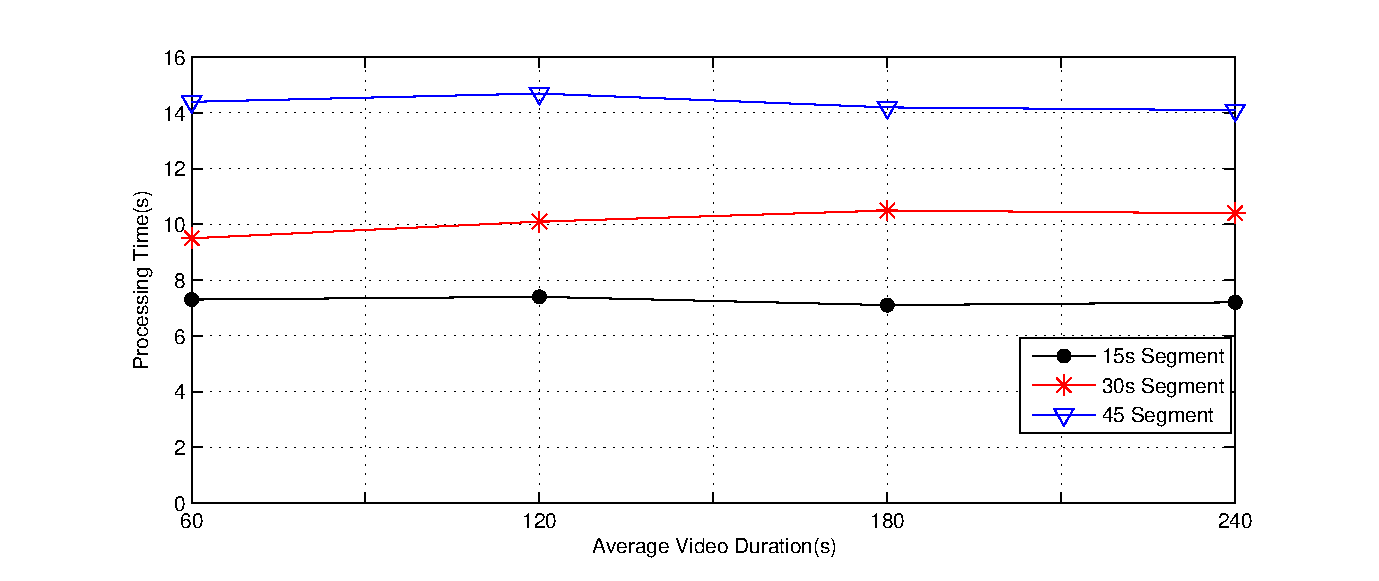
\epsfig{file=pics/videosegment.eps, height=1.7in,width=3.4in}
% %\vspace{-1mm}
% \caption{Average Video Segmentaion Time For different Duration}
% \vspace{-6mm}
% \label{fig:video}
% \end{figure}

% \textbf{Image Resize Tradeoff}
% \begin{figure*}[!t]
% \centering {
%     \subfigure[Average CEDD Execution Time Per Image for different SIZE ]{\includegraphics[width=1.6in]{pics/cedd.eps}\label{fig:resize_1}}
%     \hfil
%     \subfigure[Average Time of Resizing image to Different SIZE]{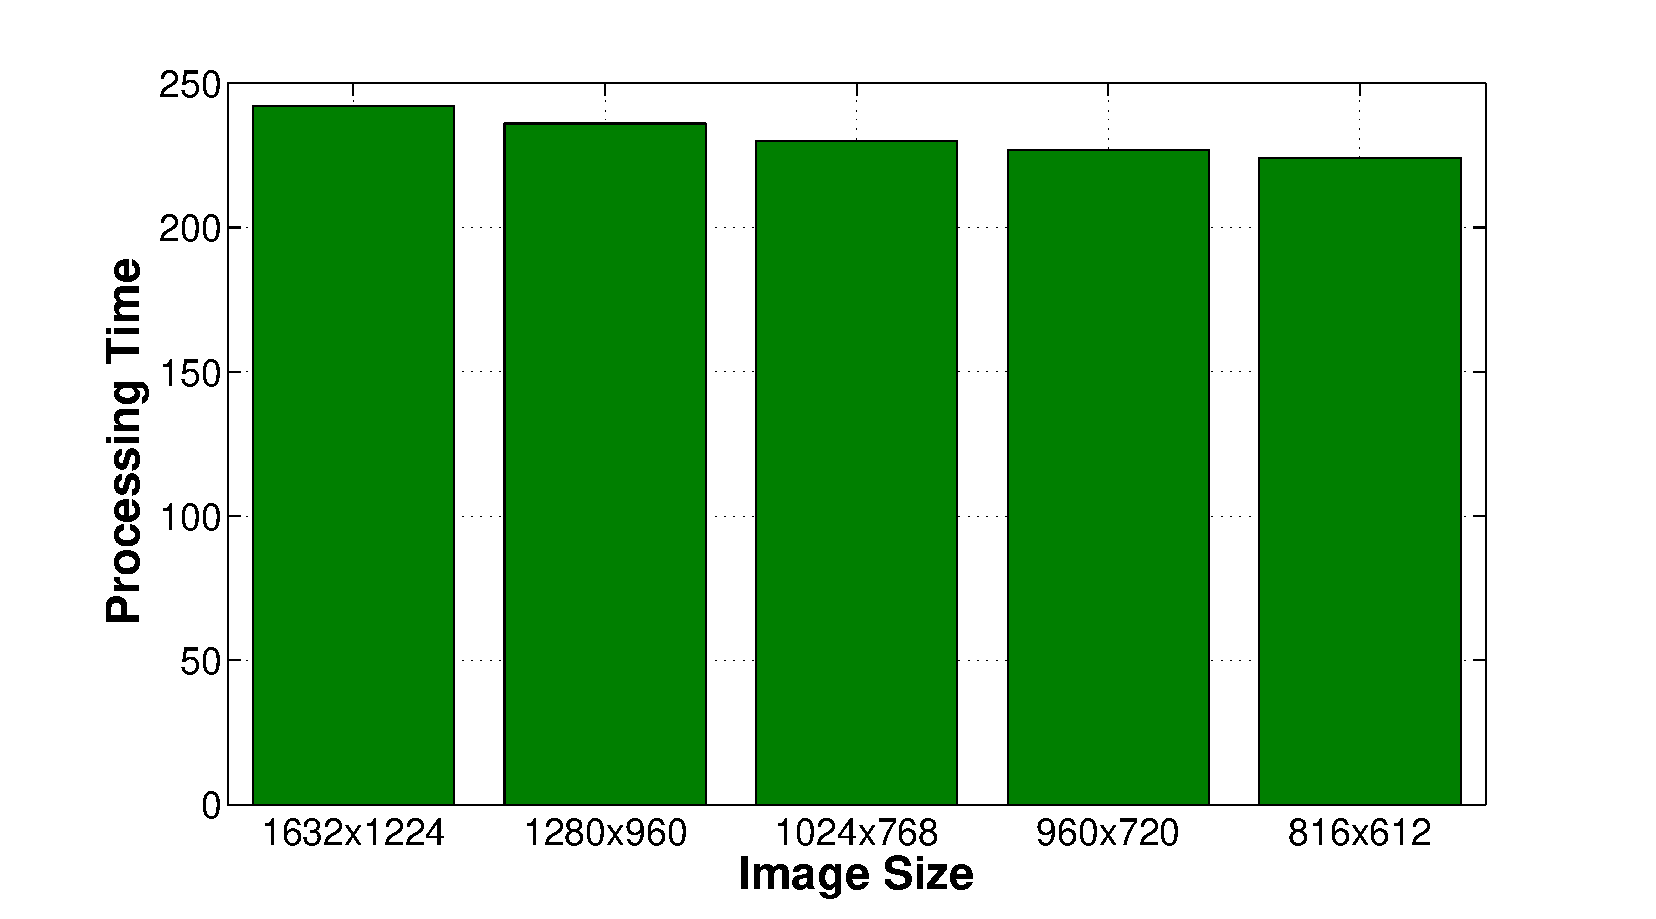
\includegraphics[width=1.6in]{pics/resizing.eps}\label{fig:resize_2}}
%     \hfil
%     \subfigure[Average Error Rate of KMeans Clustering for different Size]{\includegraphics[width=1.6in]{pics/kmeans.eps}\label{fig:resize_3}}
%     \hfil
%     \subfigure[Average Error Rate of Top K for different Size]{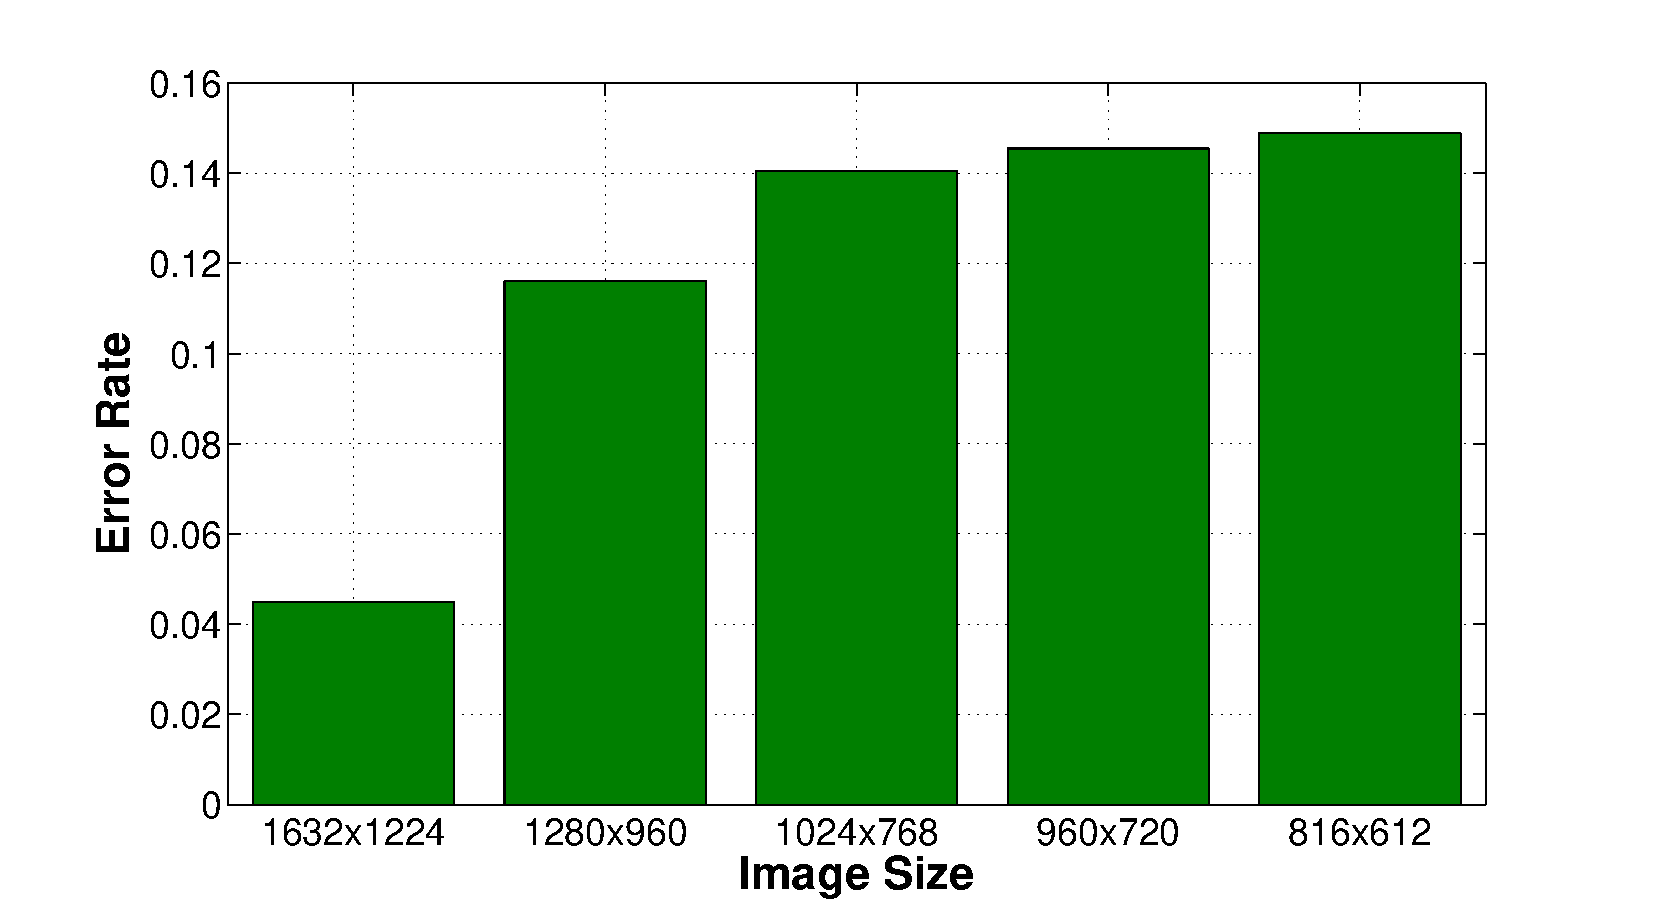
\includegraphics[width=1.6in]{pics/topk.eps}\label{fig:resize_4}}
% }
% \vspace{-1mm}
% \caption{Average Video Frame Extraction Time For Different Duration and Frequency}
% \vspace{-6mm}
% \label{fig:resize}
% \end{figure*}

% From the results, we will find 1280x960 is a good balance point here for the tradeoff of accuracy and processing time.

%\vspace*{-0.75ex}
\subsubsection{Leveraging a Crowd-Sensing Framework}
\label{sec-3-2-4}

MediaScope leverages an existing, publicly available, crowd sensing
programming framework called Medusa~\cite{Medusa}.
%
Medusa provides high-level abstractions for specifying the steps
required to complete a crowd-sensing task: in our case, uploading the
feature vectors can be modeled as a crowd-sensing task and so can the
upload of selected media objects.
%
Medusa employs a distributed runtime system that coordinates the
execution of these tasks between mobile devices and a cloud service.
%
In MediaScope, MSCloud uses Medusa to distribute tasks and collect the
results; MSMobile consists of extensions to Medusa's runtime to
implement the Feature Extractor and the Object Uploader.
%

However, in order to support MediaScope, we needed to extend the
Medusa model, which was focused on tasks generated by human users.
%
We also needed to make several performance modifications in Medusa.
%
In the former category, we modified Medusa's programming language to
selectively disable Medusa's recruitment feature and data privacy
opt-in: these features require human interaction, and
MediaScope assumes that participants have been recruited and have
signed a privacy policy out-of-band.
%
We also added a data delivery notification system that
would allow Medusa's cloud runtime to deliver notification of data
upload to external servers, such as MSCloudDB.
%
In the second category, we modified Medusa's mobile device
notification system, which originally used SMSs, to use Google's C2DM
notification service, which greatly reduced the latency of task
initiation on mobile devices.
%
We also optimized several polling loops in Medusa to be
interrupt-driven, so that we could hand-off data quickly to components
within Medusa's runtime as well as to external servers.

% to implement \mscope on Medusa, we
% need to do following modifications.
% %
% Firstly, we need to reduce the latency in Medusa system.
% %
% Medusa originally using polling-based notification indicating stage
% completed, which polls database periodically (10s) to check whether a
% stage has finished.
% %
% We add the option of directly notify Medusa server to reduce latency.
% %
% In addition, Medusa server use short message to notify smartphones to
% distribute task, we found short message delivering introduces instable
% latency, sometime over X seconds, which is not suitable for our
% timeliness query case.
% %
% To tackle this, we implement a new push notification method through
% C2DM \ref{C2DM} to reduce the notification delay.
% %
% Secondly, we can now configure a Medusa task to nitify any external
% server for particular events, for example, in a uploading task, once
% there is a new file got uploaded, Medusa can notify any specified
% external server.
% %
% Thirdly, we make Medusa server accept machine-generated tasks for
% automatic distribute tasks.
% %
% Lastly, we make the transfer component of Medusa more flexible,
% supporting different uploading schemes instead of FCFS only and the
% uploading scheme can be changed from Medusa server.
% %

% \textbf{\mscope on Medusa:} with aforementioned modification to Medusa, we can implement \mscope completely on top of it. MSCloud will periodically generate feature extraction and uploading task, which will ask all the smartphones to extract the feature of their newly captured image objects (by providing the last object id on each phone). Uploaded file containing extracted features will firstly be uploaded to Medusa server, Medusa notify MSCloud and then MSCloud parse the file and store the features in the MSCloudDB. Whenever there is a query, MSCloudQ will generate the uploading task to all the smartphones, associated with each phone's selected media objects, assigned credits and timeliness bound for the query. Then MSMobile will start to upload selected media objects based on current uploading scheme (for default OPTNAME). Once a file got uploaded to Medusa server, a notification will be sent to MSCloud, MSCloud collect such file and get prepared to return the query result page.
